\documentclass{article}

%----------------------------------------
% Packages
%----------------------------------------
\usepackage[left=1in, right=1in, top=1in, bottom=1in]{geometry}
\usepackage{graphicx}
\usepackage{amsmath,amsbsy,amssymb,amsfonts,amsthm}
\usepackage{nicefrac}
\usepackage{mathtools}
\usepackage{color}
\usepackage{xspace} % Correct macro spacing
\usepackage[numbers]{natbib} % For citations
\usepackage{times}
\usepackage{graphicx,subfigure}
%\usepackage[small,bf]{caption}
\usepackage{algorithm,algorithmic} 
\usepackage{hyperref}
\usepackage{url}

\usepackage{xcolor}
\usepackage{shadethm}

\usepackage{fancyhdr}
\pagestyle{fancy}
\lhead{This is my name}
\rhead{this is page \thepage}

\usepackage{fancyhdr}
\pagestyle{fancy}
\lhead{IFT 6085 - Theoretical principles for deep learning}
\rhead{Lecture 4: January 16, 2020}


\newshadetheorem{thm}{Theorem}
\newshadetheorem{defn}[thm]{Definition}
\newshadetheorem{assm}[thm]{Assumption}
\newshadetheorem{prop}[thm]{Property}
\newshadetheorem{eg}[thm]{Example}


\definecolor{shadethmcolor}{HTML}{F0F0F0}
%\definecolor{shadethmcolor}{HTML}{EDEDED}
%\definecolor{shadethmcolor}{HTML}{EDF8FF}
%\definecolor{shaderulecolor}{HTML}{EDF8FF}
%\definecolor{shaderulecolor}{HTML}{45CFFF}
\setlength{\shadeboxrule}{.4pt}


\setlength\parindent{0pt}

% Packages hyperref and algorithmic misbehave sometimes.  We can fix
% this with the following command.
\newcommand{\theHalgorithm}{\arabic{algorithm}}

%----------------------------------------
% Standard macros
%----------------------------------------


%----------------------------------------
% Project-specific macros
%----------------------------------------

%----------------------------------------
% Header
%----------------------------------------
\title{IFT 6085 - Lecture 4 \\ 
Black-box Models and Lower bounds }
\date{}

%----------------------------------------
% Document
%----------------------------------------
\begin{document} 

%----------------------------------------
% Abstract
%----------------------------------------
\maketitle

\vspace{-0.5in}
\begin{center}
Please report any bugs to the scribes or instructor.
\end{center}
\vspace{0.2in}

\textbf{Scribes:}
\hfill
\textbf{Instructor:} Ioannis Mitliagkas

\textbf{Winter 2020:} Etienne Thuillier

\textbf{Winter 2019:} Ian Porada, Th\'eo Moins, William Starnaud 

\textbf{Winter 2018:} Sai Krishna, Krishna Murthy 


%----------------------------------------
% Body
%----------------------------------------

\newcommand{\infgc}{\inf_{g \in \mathcal{C}}}
\newcommand{\supgc}{\sup_{g \in \mathcal{C}}}

\newcommand{\Prob}{\mathbb{P}}
\newcommand{\E}{\mathbb{E}}
\newcommand{\reals}{\mathbb{R}}


\section{Summary}

In the previous lectures, we derived upper bounds on the convergence rate of \emph{gradient descent} for minimizing different types of objective functions. Specifically, we found that depending on the properties we have for the objective function (Lipschitz-continuity, convexity, strong convexity, and smoothness), we can obtain different upper bounds on the convergence rate of gradient descent minimizing this objective function. We also saw that these different bounds are obtained with different algorithms: e.g. considering the last term of the sequence we construct, or the mean of all the points. \\

In this lecture, we will summarize these previously derived upper bounds. We will then derive a lower bound for the convergence rate of a black box model minimizing a smooth, strongly convex objective function. Our definition of black box model encompasses a class of algorithms which includes \emph{gradient descent}. \\

An upper bound on convergence rate is useful to see the efficiency of an algorithm, which is how many steps are needed to obtain a result with a given precision. In contrast, a lower bound allows us to consider the best possible upper bound we can possibly obtain for a class of algorithms. Thus, we are able to restrict ourselves in future research for a better rate of convergence: ideally models with be close this lower bound, but it would be useless to search for better.

\section{Convergence rate}

\par The upper bounds on the convergence rate of gradient descent that we have derived in this class are summarized in Table~\ref{tab:upper_bounds}. In this table $D_1 = \|x_1-x^*\|_2$, where $x_1$ denotes the initial guess, and $x^*$ the closest optimal point.

\begin{table}[H]
\centering
\renewcommand{\arraystretch}{1.8}
 \begin{tabular}{|c | c |} 
 \hline
 \textbf{Properties of the Objective Function} & \textbf{Upper bound on Convergence Rate of Gradient Descent} \\
 \hline
 convex and L-Lipschitz & $\frac{D_1L}{\sqrt{T}}$   \\ 
 \hline
 convex and $\beta$-smooth &  $\frac{\beta D_1^2}{T}$\\
 \hline
 $\alpha$-strongly convex and L-Lipschitz & $\frac{L^2}{\alpha T}$ \\
 \hline
 $\alpha$-strongly convex and $\beta$-smooth & $\beta D_1^2 \exp(-\frac{4T}{\kappa})$ \\
 \hline
\end{tabular}
\caption{Upper bounds on the convergence rate of gradient descent in relation to properties of the objective function.\label{tab:upper_bounds}}
\end{table}
\renewcommand{\arraystretch}{1}

We can see that assuming smoothness leads to a faster convergence rate as compared to the case when the objective is assumed to only be L-Lipschitz. When we assume additional properties, for instance strong convexity and smoothness, we get exponential convergence, which is our best upper bound so far. Some authors also refer to this as \emph{linear} convergence, due to the fact that a semi-logarithmic plot of the convergence rate across gradient descent iterations is reminiscent of a straight line. \\

Note that, under strongly convex and Lipschitz assumptions (i.e. third row in Table~\ref{tab:upper_bounds}), the upper bound is independent of the initial guess' distance to the optimal point. This can seem counter-intuitive. However, note that a function cannot be both strongly convex and Lipschitz-continuous globally on an unbounded domain. Indeed, strong convexity implies that the gradient increases in an unbounded fashion with distance to the optimal (think of a parabola). On the contrary, Lipschitz continuity requires that said gradient be bounded everywhere on the domain, however far from the optimal (think of a straight line). Hence, both conditions can only hold together locally within a region around the optimal point, see Fig.\ref{fig:l_lipschitz_alpha_conv}. In turn, the location of the initial guess is de facto restricted to this region, which gives an intuition as to how one can obtain a convergence upper bound formulated in terms of $\alpha$ and $L$ (which determine said region), but which is independent of the initial guess. We do not provide a more detailed treatment of this question here. See theorem 3.9 from \cite{bubeck}.

\begin{figure}[h]
    \centering
    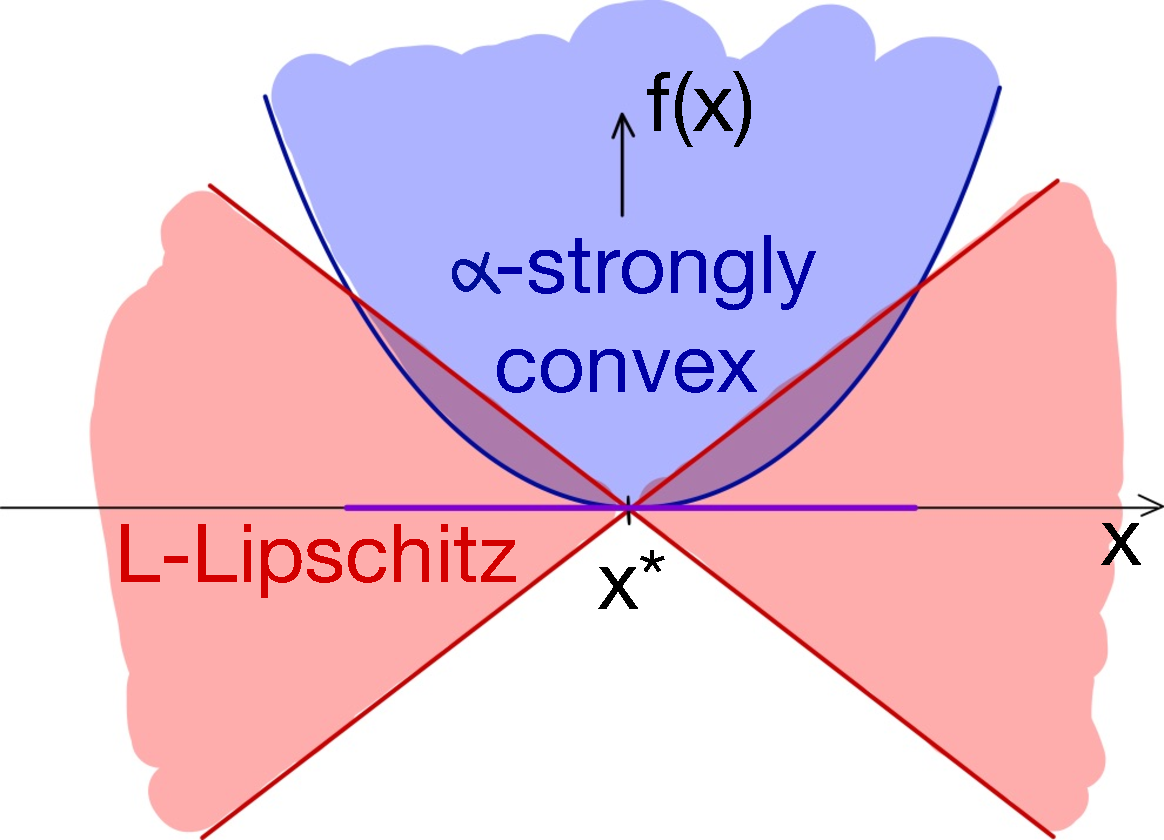
\includegraphics[scale=0.15]{img/L_Lipschitz_alpha_convex.pdf}
    \caption{The admissible domain (in purple) is compact under L-Lipschitz and $\alpha$-convex  conditions.\label{fig:l_lipschitz_alpha_conv}}
\end{figure}

\section{Black box model and taxonomy of different methods}
\label{blackbox}

A black box model assumes that the algorithm does not know the objective function $f$ being minimized.
Information about the objective function can only be accessed by querying an \emph{oracle}. The oracle serves as a bridge between the unknown objective function and the optimizer. At any given step, the optimizer queries the oracle with a \emph{guess} $x$, and the oracle responds with information about the function around $x$ (eg. value, gradient, Hessian, etc.). This model is suitable when we want to lower bound the asymptotic complexity of minimizing $f$ {\em regardless of what algorithm we use}. The complexity can be estimated as the number of queries that can be made to the oracle until we find an $\epsilon$-approximate minimum for the convex function $f$. Here we present a brief taxonomy of optimization methods, based on the nature of information about the function that the methods require.
 
\subsection{Zeroth order methods} 

These methods only require the value of function $f$ at the current guess $x$. They do not access any other \emph{higher-level} information like gradients. For example: the bisection method, genetic algorithms, simulated annealing and Metropolis method are a few techniques that {\em can} fall under this category.

\subsection{First order methods} These methods can inquire the value of the function $f$ and its first derivative (gradient or Jacobian) of the function $\nabla f$ at the current guess $x$. These methods are widely used for optimization in machine learning problems. Some of the methods include gradient descent (with or without averaging), Nesterov's accelerated gradient methods \cite{nesterov}, and Polyak's momentum \cite{polyak}.

\subsection{Second order methods} These methods require the value of the function $f$, its first derivative (gradient or Jacobian) $\nabla f$, and its second derivative (Hessian) $\nabla^2 f$ at the current guess $x$. Since these methods use information about the local curvature (which is encoded in the Hessian), they converge in a smaller number of iterations. However, each iteration is computationally intensive, as it typically involves an inversion of the Hessian. Another characteristic of these methods is the \emph{self-tuning} property. The step size (learning rate) is determined implicitly from the curvature information and need not be tuned as a hyperparameter. Newton's method is a very popular example of a second order method. \footnote{Another class of techniques, sometimes referred to as \emph{Quasi-Newton methods} is frequently used by the machine learning community. These techniques attempt to infer (approximate) second order information by using only first order information. BFGS and L-BFGS are popular Quasi-Newton methods.} Improving the efficiency of these algorithms is an active area of research.

\subsection{Adaptive methods and conjugate gradients} 

The methods we mentioned until this point assume that all dimensions of a vector-valued variable (or sometimes all variables in the objective function) have a common set of hyperparameters. \emph{Adaptive methods} relax this assumption and allow for every variable (or sometimes every dimension of a vector) to have its own set of hyperparameters (learning rate, momentum, etc). Some popular methods under this paradigm that are used in training deep neural networks are AdaGrad \cite{adagrad} and Adam \cite{adam}. \\

Conjugate gradient descent is a technique that we will not deal with in this course. But, to summarize what it does, it attains the minimum for a quadratic (exact minimum, no suboptimality) in exactly $d$ iterations, where $d$ is the dimensionality of the quadratic function. Exploiting conjugate gradients in deep network training is still an active area of research.


\newcommand{\supff}{\sup_{f \in \mathcal{F}}}

\section{Lower bounds}

Up until now, we have looked only at upper bounds on convergence rates for convex objectives that are optimized using gradient descent solvers. We will now derive a lower bound for the special case when our objective function is smooth and strongly-convex.

\subsection{Why are lower bounds useful?}

Lower bounds are useful because they tell us what's the best possible rate of convergence we can have given a category of optimizer. Without lower bounds, an unnecessary amount of research energy would be spent in designing better optimizers, even if convergence rate improvement is impossible within this category of algorithm. Caveats here are that even if we prove that each procedure has a lower bounded rate of convergence, we don't know if a specific method reaches this bound. \\

Figure \ref{conv} is a visualization of the bounds on convergence rates described thus far. As implied by comparing the slopes of these lines, our upper bounds on gradient descent describe a slower rate of convergence than the lower bounds we will derive. Upper bounds on accelerated methods' convergence rates match the derived lower bounds in all but a constant. Any convergence below the lower bound is impossible for the black box models and objective function we will describe.

\begin{figure}[h]
    \centering
    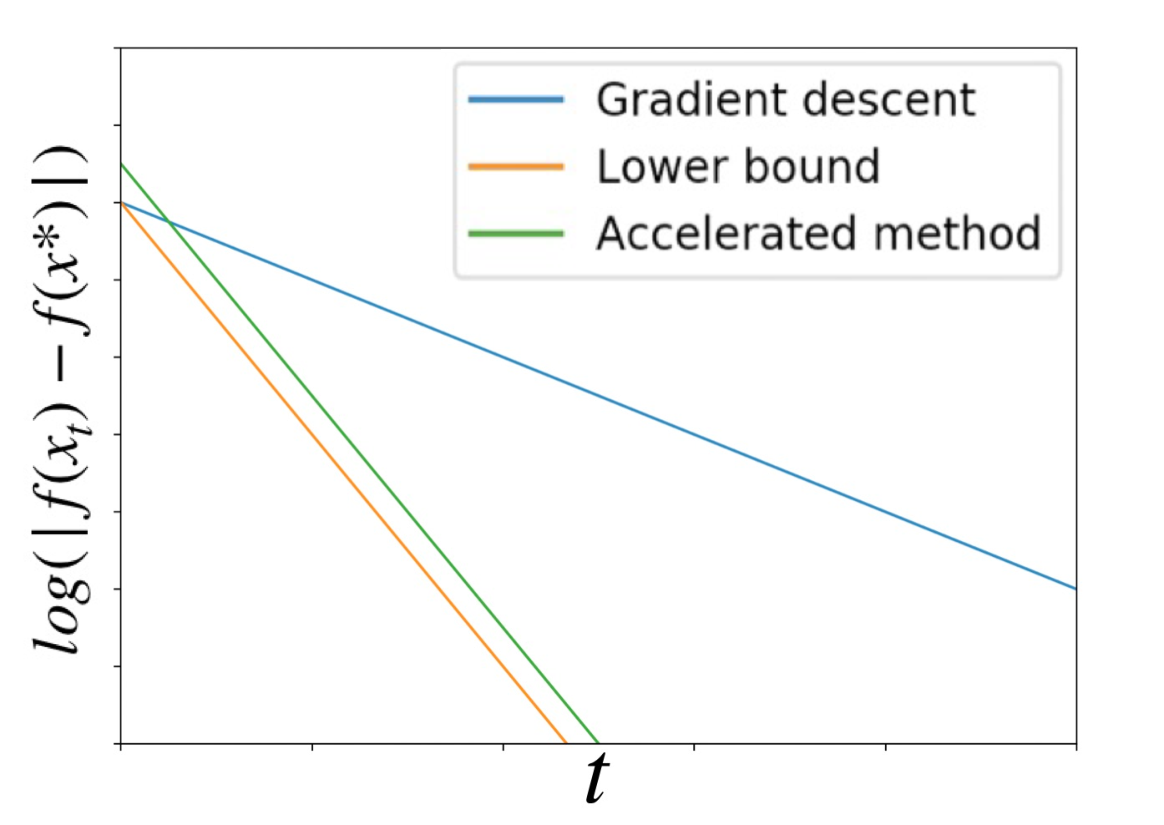
\includegraphics[scale=0.3]{img/gap.pdf}
    \caption{Converence rate for gradient descent and accelerated methods in comparison with lower bound}
    \label{conv}
\end{figure}

\subsection{Assumptions}

Under the black box model for first-order methods, we consider a sequence of iterates $x_1, x_2, x_3, ...$ and a sequence of gradients $g_1, g_2, g_3, ...$. The optimizer updates the variable $x$ (interchangeably referred to as the parameter vector) using an update rule that satisfies the following criterion:
\begin{equation*}
    x_{t+1} \in span\left( g_1, g_2, ..., g_t \right)
\end{equation*}

This means that $x_{t+1}$ must be a linear combination of the sequence of gradients computed thus far in the algorithm. Here, $t$ is an index into the number of steps the optimizer is run for. Further, in our analysis, we assume that the initial guess $x_1$ is always the zero vector ($x_1 = \mathbf{0}$), without loss of generality. The above model can easily be tweaked to hold for arbitrary initializations, but in that case, expressions for bounds become tedious. We only make this assumption for algebraic simplicity, because we are interested in bounds on asymptotic rates. \footnote{If the initial guess was not the zero vector, but $x_{init}$, the update rule criterion must be modified to $x_{t+1} \in span\left( x_{init}, g_1, g_2, ..., g_t \right)$}

\subsection{Lower bounds for smooth and strongly convex objectives}

Now, we proceed to derive a lower bound for an objective function which is $\alpha$-strongly convex and $\beta$-smooth. Before we proceed, we outline some notation that will be used in the proof. \\

%The \emph{condition number} for a matrix will be denoted by $\kappa$. It is the ratio of the largest singluar value of the matrix to its smallest singluar value. If the condition number of a matrix is infinity, then the corresponding linear system is termed \emph{singular}. If the condition number is too large (but not infinity), then the corresponding linear system is termed \emph{ill-conditioned} (or \emph{poorly conditioned}). \\

\begin{thm}
(Theorem 3.15 from \cite{bubeck})
($\kappa >  1$) There exists a $\beta$-smooth and $\alpha$-strongly convex function $f \colon l_2 \mapsto \mathbb{R}$ with condition number $\kappa = {\beta \over \alpha}$ such that for any $t \geq 1$ and any \emph{black box} procedure (see Section \ref{blackbox}), the following lower bound holds.

\begin{equation}
f(x_t) - f(x^*) \geq {\alpha \over 2}  \left( \frac{\sqrt[]{\kappa} - 1}{\sqrt[]{\kappa} + 1} \right)^{2(t-1)}  ||x_1 - x^*||^2
\end{equation} \\
for large values of $\kappa$, \\
\begin{equation}
 \left(\frac{\sqrt[]{\kappa} - 1}{\sqrt[]{\kappa} + 1} \right)^{2(t-1)} \approx \exp{ \left(-\frac{4(t-1)}{\sqrt[]{\kappa}}\right)}
\end{equation}

\end{thm}


\begin{proof}

As is typical of lower bound proofs, we prove this theorem by constructing an example. The example function we construct is an $\ell_2$ function. Informally speaking, $\ell_2$ functions are vectors with infinitely many coordinates that are also square summable. Formally, 
	\[\ell_2 = \{ x = (x(n)), n \in \mathbb{N}, \sum_{i=1}^{\infty} x(i)^2 < +\infty \}\]
    
We define an operator that assumes the form of a tridiagonal matrix. Let
	\[ A = \left[ \begin{matrix} 2 & -1 & 0 & \dots & \dots & \dots & \dots & \dots & \dots \\ -1 & 2 & -1 & 0 & \dots & \dots & \dots & \dots & \dots \\ 0 & -1 & 2 & -1 & 0 & \dots & \dots & \dots & \dots \\ \vdots & 0 & -1 & 2 & -1 & 0 & \dots & \dots & \dots \\ \vdots & \vdots & 0 & -1 & 2 & -1 & 0 & \dots & \dots \\ \vdots & \vdots & \ddots & \ddots & \ddots & \ddots & \ddots & \ddots & \vdots  \end{matrix} \right] \] \\
    
This operator has all its eigenvalues in the range [0,4].  This can be found by the use of Gershgorin disks\footnote{\url{https://en.wikipedia.org/wiki/Gershgorin_circle_theorem}}. First, we let $R_i = \sum_{j \neq i} |a_{ij}|$. Then we define the Gershgorin discs $D(a_{ii},R_i)$ of A as $D(a_{ii},R_{i}) = \left\{z\in {\mathbb  {C}},|a_{{ii}}-z|\leq R_i\right\}$. The Gershgorin circle theorem \cite{Ger31} then states that every eigenvalue of A must lie within at least one the discs $D(a_{ii},R_i)$.

So with our expression of A, we only have two different discs, namely $D(2,1)$ and $D(2,2)$. The firs one is included in the latter one (i.e. $D(2,1) \subset D(2,2)$). Moreover, A is symmetrical, so the eigenvalues of A are real. We can infer that the eigenvalues of A must be in $[0,4]$.\\

Thus, we can define the following quadratic function:
	\[f(x) = {\alpha(\kappa-1) \over 8} \left( \langle Ax,x\rangle - 2\langle e_1,x \rangle \right) + {\alpha \over 2} \|x\|^2\]
	Here, $\langle .,. \rangle$ denotes the vector inner-product and $e_1$ denotes the first vector of the canonical basis, i.e., \[e_1 = \left[ 1,0,0, \dots \right]^T.\]
    
Since $A$ is symmetric by definition,
\[	\langle Ax,x \rangle = x^TA^Tx = x^TAx \]

Also note that $f$ is $\alpha$-strongly convex (the ${\alpha \over 2} \|x\|^2$ term ensures that) and $\beta$-smooth. $\beta$-smoothness arises from the property that the eigenvalues of $A$ are bounded to be in the range $\left[ 0,4 \right]$. We now compute the gradient of $f$.
\[
\nabla f(x) = {\alpha (\kappa-1) \over 4} \left( Ax - e_1 \right) + \alpha x
\]    

Recall that, under the black box model we assumed that the starting point for our gradient descent routine will be $x_1 = 0$. Plugging that into the expression above, we get
\[
\nabla f(x)_{x = x_1} = -{\alpha (\kappa-1) \over 4} e_1 = \left[ \begin{matrix}
	-\alpha (\kappa-1) \over 4 \\ 0 \\ 0 \\ \vdots
	\end{matrix} \right]
\]

Using this expression, it is easy to show---by mathematical induction---that if $x_{t-1}$ has non-zero entries up to element at index $t-1$, then $x_{t}$ will have non-zero entries up to index $t$.
The way the Hessian $A$ is designed, the non-zero values propagate across the dimensions, one dimension per each step of the gradient descent routine.

That is, $x_t(i) = 0 \ \forall i \geq t$. Let's now consider the norm
\begin{equation}\label{normsumeq}
	\begin{alignedat}{2}
	\|x_t - x^*\|^2 & = \sum_{i=1}^{\infty} \left( x_t(i) - x^*(i) \right)^2 &&\\
	 & = \sum_{i=1}^{t-1} \left( x_t(i) - x^*(i) \right)^2 + \sum_{i=t}^{\infty} \left( x_t(i) - x^*(i) \right)^2 \ && \textnormal{(separating the non-zero entries)} \\
	  & = C + \sum_{i=t}^{\infty} \left( x_t(i) - x^*(i) \right)^2 &&\textnormal{(with $C > 0$)} \\
	  & \geq \sum_{i=t}^{\infty} \left( x_t(i) - x^*(i) \right)^2 &&\textnormal{(the first term above was positive)} \\
	   & = \sum_{i=t}^{\infty} \left(x^*(i) \right)^2 && \textnormal{(all terms are zeros, beginning from term $t$)}
	\end{alignedat}
\end{equation}
    
Of course, as we keep running gradient descent, $\|x_t\|$ keeps getting smaller and smaller (if the learning rate is appropriately specified). Strong convexity gives us

\begin{equation}
	\begin{split}
	f(x_t) - f(x^*) & \geq {\alpha \over 2} \| x_t - x^* \|^2 \\
	 & \geq {\alpha \over 2} \sum_{i=t}^{\infty} \left( x^*(i) \right)^2
	\end{split}
\end{equation}

If we differentiate $f$ and set $\nabla f$ to $0$, we obtain an infinite linear system, of the following form (using the definition of $A$):
\begin{equation}\label{linsys}
    \left\{
	\begin{aligned}
		& 1 - 2{\kappa + 1 \over \kappa - 1}x^*(1) + x^*(2) = 0, \\
        & x^*(k-1) - 2{\kappa + 1 \over \kappa - 1}x^*(k) + x^*(k+1) = 0 \ \forall k \geq 2.
	\end{aligned}
	\right.
\end{equation}
The solution of the above system is given by
\[
x^*(i) = \left( \sqrt{\kappa}-1 \over \sqrt{\kappa}+1 \right)^i
\]
\emph{Hint for derivation:} We sum all rows in the linear system to obtain $1 - x^*(1) + \sum_{k=1}^\infty [2 - 2({\kappa+1 \over \kappa -1})]x^*(k)=0$. We put $x^*(k)=r^k \ \forall k \geq 1$ and we use the value of geometric series to solve for $r$. \\
\\
Now, we plug this into the above expression, which gives us
\begin{equation}
	\begin{alignedat}{2}
	f(x_t) - f(x^*) & \geq {\alpha \over 2} \| x_t - x^* \|^2  &&\\
	 & \geq {\alpha \over 2} \sum_{i=t}^{\infty} (x_t^*(i))^2 &&\\
	  & = {\alpha \over 2} \sum_{i=t}^{\infty}  \left( \sqrt{\kappa}-1 \over \sqrt{\kappa}+1 \right)^{2i} && \text{(By solution to the linear system ($\ref{linsys}$) above)}\\
	  & = {\alpha \over 2} \sum_{i=1}^{\infty}  \left( \sqrt{\kappa}-1 \over \sqrt{\kappa}+1 \right)^{2(i+t-1)} &&\text{(By change of variable)}\\
	  &= \frac{\alpha}{2}\left({\sqrt{\kappa} - 1 \over \sqrt{\kappa} + 1}\right)^{2(t-1)} \sum_{i=1}^\infty \left({\sqrt{\kappa} - 1 \over \sqrt{\kappa} +1}\right)^{2i} &&\\
	  &= \frac{\alpha}{2} \left( \sqrt{\kappa} - 1 \over \sqrt{\kappa} + 1 \right)^{2(t-1)} \sum_{i=1}^{\infty} \left( x^*(i) \right)^{2} && \text{(By solution to the linear system ($\ref{linsys}$) above)}\\
	  & = {\alpha \over 2} \left( \sqrt{\kappa}-1 \over \sqrt{\kappa}+1 \right)^{2(t-1)}||x_1 - x^*||^2 && \text{(By derivation ($\ref{normsumeq}$) above for $x_1$)}
	\end{alignedat}
\end{equation}

This proves the theorem.

\end{proof}


\newcommand{\cf}{\mathbb{S}_{\mathcal{F}}}



%----------------------------------------
% \section*{Acknowledgments} 

%----------------------------------------
\bibliographystyle{abbrvnat}
\bibliography{Refs/lec4}

%----------------------------------------
\end{document}
